\documentclass[journal=jprobs,manuscript=article]{achemso}
\usepackage[utf8]{inputenc}
\usepackage{amsmath}
\usepackage{hyperref}
\usepackage[dvipsnames]{xcolor}
%\usepackage{authblk}

%\usepackage{changepage}   % For adjusting image width

%%%%%%%%%%%%%%%%%%%%%%%%%%%%%%%%%%%%%%%%%%%%%%%%%%%%%%%%
% Removed dependency on the Supplemental file, manually labeled all supplemental figures in the manuscript.

%%% HELPER CODE FOR DEALING WITH EXTERNAL REFERENCES
%  This snippet of code lets us reference figures from the supplements
%       in the main text. This can easily be removed once the
%       supplementary numbering is stable.
%
%  Tested in Overleaf and in MiKTeX 2.9
%\usepackage{xr}
%\makeatletter
%\newcommand*{\addFileDependency}[1]{% argument=file name and extension
%  \typeout{(#1)}
%  \@addtofilelist{#1}
%  \IfFileExists{#1}{}{\typeout{No file #1.}}
%}
%\makeatother

%\newcommand*{\myexternaldocument}[1]{%
%    \externaldocument{#1}%
%    \addFileDependency{#1.tex}%
%    \addFileDependency{#1.aux}%
%}
%%% END HELPER CODE



%%% Looks for the supplementary figure document to cocompile for
%%% supplementary figure numbering
%\myexternaldocument{supplement_figs}
%%%%%%%%%%%%%%%%%%%%%%%%%%%%%%%%%%%%%%%%%%%%%%%%%%%%%%%%%

\title{Mouse primary T cell phosphoyrosine proteomics enabled by BOOST}
\author{Xien Yu Chua$^{1,\P}$, Kenneth P. Callahan$^{2,\P}$, Alijah A. Griffith$^{2}$, Tobias Hildebrandt$^{1}$, Guoping Fu$^{3}$, Mengzhou Hu$^{1}$, Renren Wen$^{3}$, Arthur R. Salomon$^{2,*}$
\\
\singlespacing
\textit{\small{$1$ Department of Molecular Pharmacology, Physiology \& Biotechnology, Brown University, Providence, RI, 02912}}
\\
\textit{\small{$2$ Department of Molecular Biology, Cell Biology \& Biochemistry, Brown University, Providence, RI, 02912}}
\\
\textit{\small{$3$ Blood Research Institute, Blood Center of Wisconsin, Milwaukee, WI, 53226}}
\\
\textit{\small{$\P$ Contributed equally to this work}}
\\
\textit{\small{$*$} Corresponding Author}\tiny}
\email{art@drsalomon.com}
%
%
% In our previous manuscript submission using LaTeX (https://doi.org/10.1021/acs.jproteome.1c00735),
% The editors of JPR wanted the author affiliations to be numbered, rather than
% the symbols automatically provided by the achemso package. 
%
% To get back to the original code, just comment out the lines above and uncomment the
% lines below.

%\author{Xien Yu Chua}
%\altaffiliation{Contributed equally to this work}
%\affiliation{Department of Molecular Pharmacology, Physiology \& Biotechnology, Brown University, Providence, RI, 02912}
%\author{Kenneth P. Callahan}
%\altaffiliation{Contributed equally to this work}
%\author{Alijah A. Griffith}
%\affiliation{Department of Molecular Biology, Cell Biology \& Biochemistry, Brown University, Providence, RI, 02912}
%\author{Tobias Hildebrandt}
%\affiliation{Department of Molecular Pharmacology, Physiology \& Biotechnology, Brown University, Providence, RI, 02912}
%\author{Guoping Fu}
%\affiliation{Blood Research Institute, Blood Center of Wisconsin, Milwaukee, WI, 53226}
%\author{Mengzhou Hu} 
%\affiliation{Department of Molecular Pharmacology, Physiology \& Biotechnology, Brown University, Providence, RI, 02912}
%\author{Arthur R. Salomon}
%\email{art@drsalomon.com}
%\affiliation[Brown University]{Department of Molecular Biology, Cell Biology \& Biochemistry, Brown University}


\date{January 2022}
%
%
%%%%%%%%%%%%%%%%%%%%%%%%%%%%%%%%%%%%%%%%%%%%%%%%%%%%%%%%%%%%%%%%%%%%%%%%%%%%%%%%%%%%%%%%%%


\begin{document}



\maketitle

\begin{tocentry}

For TOC only

\includegraphics{figures/graphical_toc/mouse_turbotmt_gtoc.pdf}
\end{tocentry}

%https://texdoc.org/serve/achemso.pdf/0
%\singlespacing

\begin{abstract}

The Broad Spectrum Optimization of Selective Triggering (BOOST) approach was recently developed to increase the quantitative depth of the tyrosine phosphoproteome by mass spectrometry-based proteomics. While BOOST has been demonstrated in the Jurkat T cell line, it has not been demonstrated in scarce mice primary T cells. Here, we show the first phosphotyrosine proteomics experiment performed in mice primary T cells using BOOST. We identify and precisely quantify more than $3{,}000$ unique pTyr PSMs using only $1$ mg of protein from T cell receptor-stimulated primary T cells from mice. We further reveal the importance of the phase-constrained spectrum deconvolution method ($\Phi$SDM) parameter on Orbitrap instruments that, when disabled, enhances quantitation depth, accuracy, and precision in low-abundance samples. Using samples with contrived ratios, we find that disabling $\Phi$SDM allows for up to a two-fold increase in the number of statistically significant intensity ratios detected while enabling $\Phi$SDM degrades quantitation, especially in low-abundance samples.


\end{abstract}

Keywords:

\begin{itemize}
    \item {\textbf{Mice}}
    \item {\textbf{T cell}}
    \item {\textbf{BOOST} }
    \item {\textbf{TMT} }
    \item {\textbf{SH2 superbinder}}
    \item {\textbf{Phosphotyrosine proteomics} }
    \item {\textbf{Phase-constrained spectrum deconvolution method}}
\end{itemize}

\section{Introduction}

% Paragraph 1: Tyrosine phosphorylation and importance for T cells

Kinase signaling cascades regulate key cellular processes including growth, differentiation, and trancsriptional regulation. In T cells, binding of antigen-loaded peptide major histocompatibility complex on antigen-presenting cells to the T cell  receptor (TCR) initiates early tyrosine kinase-mediated signaling, leading to serine/threonine kinase activation that regulates transcriptional activation\cite{gaud2018regulatory}. Signal initiation from the TCR begins via recruitment of the Src family tyrosine kinases Lck and Fyn, which phosphorylate tyrosine residues in immunotyrosine activation motifs (ITAMs) on the intracellular domain of TCR complex subunits TCR$\zeta$, CD3$\epsilon$, CD3$\delta$, and CD3$\gamma$\cite{palacios2004function,gaud2018regulatory}. Next, the Syk-family tyrosine kinase Zap70 binds to phosphorylated ITAMs, is itself phosphorylated by TCR-proximal Lck, and directed toward substrates associated with the critical scaffolding protein linker for activation of T cells (LAT) by Lck\cite{lo2018lck}. Zap70 and the Lck-activated Tec-family tyrosine kinase Itk phosphorylate and activate many LAT-associated proteins, culminating in serine/threonine kinase activation upstream of cytokine expression and actin cytoskeletal regulation\cite{gaud2018regulatory,kumari2014t}. Despite the importance of tyrosine phosphorylation in the early stages of TCR signaling, tyrosine phosphorylation is scarce, accounting for less than $1\%$ of all phosphorylation events\cite{hunter1980transforming,hunter2009tyrosine}.% compared to serine/threonine phosphorylation.

% Parargraph 2: Sequencing limitations in primary cells 

Due to the scarce nature of tyrosine phosphorylation, large-scale phosphotyrosine (pTyr) proteomic studies of TCR signaling in mice primary T cells are often impaired by low yield. Recently, \citeauthor{locard2020lymphoatlas} performed a phosphoproteomic study by antibody-stimulating $100$ million CD4$^{+}$ T cells per replicate before phophotyrosine enrichment using the pTyr-$1000$ enrichment kit. Using this approach, \citeauthor{locard2020lymphoatlas} identified a total of $254$ unique pTyr sites from $786$ unique pTyr peptides, which is comparable to phosphoproteomic studies of TCR and chimeric antigen receptor signaling in primary human T cells\cite{joshi2017phosphoproteomics,salter2021comparative,ramello2019immunoproteomic}. Phosphotyrosine-specific enrichment methods provide improved pTyr sequencing compared to the more commonly used global phosphopeptide enrichment strategies like immobilized metal affinity chromatography (IMAC) or titanium dioxide (TiO$_{2}$)\cite{navarro2011phosphoproteomic,prado2021synergistic}. One phosphoproteomic study of TCR signaling in mice using $20$ million cells per replicate and IMAC phosphopeptide enrichment identified only $77$ unique pTyr peptides \cite{iwai2010quantitative}, whereas other studies report $1$-$2\%$ (about $250$ to $700$) of their total yield as unique pTyr peptides using IMAC or TiO$_{2}$\cite{alvarez202023,navarro2011phosphoproteomic}. As demonstrated in \citeauthor{iwai2010quantitative}, decreasing the number of cells and therefore the amount of protein input can severely limit pTyr quantitation depth in primary T cells from mice. 

%In a recent phosphoproteomics study comparing TCR and chimeric antigen receptor (CAR) signaling in primary human T cells, \citeauthor{salter2021comparative} identified a combined total of $715$ unique tyrosine phosphorylation sites from both TCR- and CAR-stimulated primary human cells\cite{salter2021comparative}. 

%While the number of unique pTyr sites are higher than other comparable studies in primary cells\cite{iwai2010quantitative,ramello2019immunoproteomic}, experimentally equivalent pTyr proteomic studies of TCR signaling in Jurkat T cells, a human leukimic T cell line and an established model of TCR signaling\cite{abraham2004jurkat}, have consistently yielded between of $250$ and $1{,}500$ unique pTyr sites\cite{cao2012quantitative,ji2015src,griffith2021silac,belmont2017plc}.

 %For this reason, many phosphotyrosine proteomic studies of T cell signaling are performed in the Jurkat human leukemic cell line\cite{}.

%Our current understanding of TCR signaling is largely based on studies in Jurkat T cells, a T cell lymphoma cell line that is easy to genetically manipulate and culture in large quantities.

% Paragraph 3: Wet and Computational methods to improve quantitation

To increase the accuracy, precision, and reporducibility of pTyr quantitation in cases of limited protein availability, both experimental and computational approaches are being developed. For example, recent improvements in pTyr enrichment reagents, namely the superbinder SH2 enrichment method\cite{kaneko2012superbinder,bian2016ultra,dong2017sensitive,tong2017protein,yao2018sh2,yao2019one}, have improved quantitation depth of the pTyr proteome\cite{chua2020tandem,chua2021ovalbumin,griffith2021silac}. Additionally, the use of isobaric labeling reagents like tandem mass tags (TMT) have allowed for accurate phosphopeptide quantitation in multiplexed samples with a higher probability of identifying unique peptides compared to label-free quantitation\cite{thompson2003tandem,wiese2007protein,werner2012high,mcalister2012increasing,o2018proteome,thompson2019tmtpro}. To improve the spectral quality and speed of acquiring TMT samples on Fourier transfrom-mass spectrometers (FT-MS), instrument settings like the phase-constrained spectrum deconvolution method ($\Phi$SDM) are available. By applying the $\Phi$SDM, FT spectra are deconvolved into frequency distributions, allowing for efficient extraction of the harmonic components of oscillating ions and ultimately achieving higher mass accuracy and resolution in shorter times\cite{grinfeld2017phase}.

% Paragraph 4: What we do

Recently, we combined the multiplexing capability of TMT, the selectivity of superbinder SH2, and a carrier channel using broad phosphatase inhibnition to develop the broad-spectrum optimization of selective triggering (BOOST) method to increase pTyr quantitation depth in proteomics experiments\cite{chua2020tandem}. During the development of BOOST we used Jurkat T cells, a model system for studying TCR signaling\cite{abraham2004jurkat}. However the BOOST method has not yet been demonstrated in the more biologically relevant primary T cells from mice. Here, we report the first pTyr proteomics study in primary T cells from mice using the BOOST method. By using predetermined protein input amounts, we show that BOOST increases the sequencing depth of low abundance samples, yielding more than $3{,}000$ unique pTyr peptides in experimental samples. We also show that acquiring samples using the $\Phi$SDM degrades quantitation in low-abundance samples. By using samples with contrived ratios, samples acquired with the $\Phi$SDM disabled have higher replicate reproducibility, are more accurate, and are more precise than equivalent samples acquired with the $\Phi$SDM enabled.

\section{Materials and Methods}



\subsection{Stimulation of mice primary T cells}

CD8$+$ thymocytes from B6 mice were harvested and blasted in cell culture using IL-2. Cells were rested in $1\%$ BSA T cell media for $2$ hours at $2\times 10^6$ cells/ml prior to stimulation. To initiate T cell stimulation, $25 \ \mu$g/mL of biotin-labeled $\alpha$-CD3 antibody (Clone $<$ C305?$>$ and $25 \ \mu$g/mL streptavidin were added to the cells resuspended at $1\times 10^8$ cells/ml for $5$ minutes at $37^{\circ}$C. After $5$ minutes of stimulation, cells were lysed with 1\% (w/v) sodium dodecyl sulfate (SDS) in $100$ mM Tris-HCl (pH $7.6$). Pervanadate treatment for the carrier channel sample was performed by incubating cells with $500 \ \mu$M PV (prepared by mixing equal volume of $1$ mM sodium orthovanadate and $1$ mM hydrogen peroxide) for $20$ minutes at $37^{\circ}$C.

\subsection{Sample processing}

Lysate was applied through QIAshredder Mini Spin Column by centrifugation at $20{,}000\times$g at $37^{\circ}$C for $5$ minutes. Protein concentration was determined using Pierce BCA Protein Assay (Thermo Fisher Scientific, 23225), after which it was reduced by $100$ mM dithiothreitol at room temperature for $30$ minutes. Lysate was subsequently processed and digested using the filter-aided sample preparation (FASP) method\cite{wisniewski2009universal} as described previously. Digested peptides were collected and acidified by trifluoroacetic acid and desalted using Sep-Pak C18 Cartridge (Waters WAT020515) as described previously\cite{ahsan2017quantitative}. Desalted peptides were labeled using a Tandem Mass Tag as described previously\cite{chua2020tandem}. TMT-labeled peptides were mixed and purified for phosphotyrosine peptides using the Src SH2 domain superbinder as described previously\cite{chua2020tandem}.

\subsection{Liquid chromatography tandem mass spectrometry}

Offline basic (pH $10$) fractionation of peptides was performed on a $100$ mm $\times$ $1.0$ mm Acquity BEH C18 column (Waters) using an UltiMate $3000$ UHPLC system (ThermoFisher Scientific) with a $40$-minute gradient from $1\%$ to $40\%$ Buffer B$_{\text{basic}}$ into $36$ fractions. The $36$ fractions were subsequently consolidated into $12$ super-fractions (Buffer A$_{\text{basic}}$ = $10$ mM ammonium hydroxide in $99.5\%$ (v/v) HPLC-grade water, $0.5\%$ (v/v) HPLC-grade acetonitrile; Buffer B$_{\text{basic}}$ = $10$ mM ammonium hydroxide in $100\%$ HPLC-grade acetonitrile), which were further separated on an in-line $150$ mm $\times$ $75 \ \mu$m reversed phase analytical column packed in-house with XSelect CSH C18 $2.5\ \mu$m resin (Waters) using an UltiMate $3000$ RSLCnano system (ThermoFisher Scientific) at a flow rate of $300$ nL/min. Peptides were then eluted using a $65$-minute gradient from $5\%$ to $30\%$ Buffer B$_{\text{acidic}}$, followed by a $6$-minute gradient $30\%$ to $90\%$ Buffer B$_{\text{acidic}}$ (Buffer A$_{\text{acidic}}$ = $0.1\%$ (v/v) formic acid in $99.4\%$ (v/v) HPLC-grade water, $0.5\%$ (v/v) HPLC-grade acetonitrile; Buffer B$_{\text{basic}}$ = $0.1\%$ (v/v) formic acid in $99.9\%$ (v/v) HPLC-grade acetonitrile). Data were acquired in data-dependent acquisition (DDA) mode on a Orbitrap Eclipse Tribrid mass spectrometer (ThermoFisher Scientific) with a positive spray voltage of $2.25$ kV, multinotch TMT-MS3 settings,\cite{mcalister2014multinotch} and a cycle time was set at 2.5 seconds. At the MS1 level, precursor ions with charge states from $2$ to $5$ were acquired on the Orbitrap detector with a scan range of $400-1600$ $m/z$, $120{,}000$ resolution, maximum injection time of $50$ ms, automatic gain control (AGC) target of $800{,}000$, and a dynamic exclusion time of $15$ seconds. An isolation window of $0.7$ $m/z$ was used to isolate MS1 precursor ions on the quadrupole for MS2 scans. MS2 scans were acquired in centroid mode on the ion trap detector on a scan range of $400-1400$ $m/z$ via higher-energy dissociation (HCD, $33\%$ energy) activation with an AGC target of $5000$, maximum injection time of $75$ ms. Using synchronous precursor selection (SPS)\cite{mcalister2014multinotch}, $10$ notches were further isolated on the quadrupole using an MS2 isolation window of $3$ $m/z$ for MS3 scans, which are acquired on the Orbitrap detector on a scan range of $100-500$ $m/z$ in a mass resolution of $50{,}000$ via HCD activation ($55\%$ energy) with a AGC target of $250{,}000$ and maximum injection time of $150$ ms in centroid mode.

\subsection{Database Search Parameters and Acceptance Criteria for Identifications}

Raw files were processed in MaxQuant\cite{cox2008maxquant} version $1.6.17.0$ using the integrated peptide search engine Andromeda\cite{cox2011andromeda}. MS/MS spectra were searched against a mouse UniProt database (Mus musculus, last modified 12/01/2019) comprised of $55{,}412$ forward protein sequences. False discovery rate (FDR) for peptide spectrum matches (PSM) was set at $1\%$ using a reverse decoy database approach. Carbamidomethylation (cysteine) was set as fixed modification, whereas oxidation (methionine), acetylation (protein N-termini) and phosphorylation (serine, threonine, tyrosine) were set as variable modifications. Trypsin enzyme specificity was used with up to $2$ missed cleavages. Main search peptide tolerance was set as $5$ ppm, while FTMS and ITMS MS/MS match tolerances were set as $20$ ppm and $0.5$ Da, respectively. MS3 reporter ion mass tolerance was set at $3$ mDa, using isotopic correction factors provided by the manufacturer (Lot UK291564, Lot UH283151). The search parameter fil (mqpar.xml) and all MaxQuant output files are provided in Supporting Folder $1$.

\subsection{Data Analysis \& Code Availability}

All analysis and data visualization were preformed on Ubuntu $20.04$ LTS in the Windows Subsystem for Linux version $2$ using Python $3.8.10$ with the packages ``Matplotlib" (Version $3.3.2$), ``SciPy" (Version $1.7.3$), ``pandas" (Version $1.2.3$), ``NumPy" (Version $1.19.2$), ``Biopython" (version $1.78$), and ``matplotlib-venn" (version $0.11.6$) and is available in Supporting Folder $1$. Analysis of unique PSMs was performed using the MaxQuant output file ``evidence.txt" (Supporting Folder $2$). Unique PSMs were defined by a non-redundant amino acid sequence (including posttranslational modifications), the charge state of the peptide, and the least number of missing values across all TMT channels. In the cases where redundancy was still present, we kept the peptide with the highest median reporter intensity. For assigning flanking sequences to each peptide and generating Supporting Figure $1$, the MaxQuant output file ``Phospho (STY)Sites.txt" (Supplementary Folder $2$) was used. For determining previously annotated pTyr sites we used the PhosphoSitePlus$^{\text{\textregistered}}$ (\href{www.phosphosite.org}{www.phosphosite.org})\cite{hornbeck2015phosphositeplus} posttranslational modification database file ``Phosphorylation\_site\_dataset.txt" (Supporting Folder $1$). Before analysis, all peptides at a $1\%$ FDR flagged as ``potential contaminants" or ``reverse hits" were removed, and reporter ions from the PV-treated sample (TMT126) and the Blank channel (TMT127N) were excluded from further analysis unless otherwise stated. Statistical significance between the mean corrected reporter intensities for $1.0$ mg, $0.3$ mg, and $0.1$ mg protein input samples was determined using unpaired Student's T-tests to calculate $p$-values before correcting for multiple hypotheses (generating $q$-values) using the method of Benjamini \& Hochberg\cite{benjhoch}. For all comparisons, statistical significance was only attained for peptides where reporter intensity values were present for all three replicates. In line with the previous literature, we did not impute or interpolate missing values at any point during data analysis\cite{chua2020tandem,chua2021ovalbumin}. To evaluate replicate reproducibility, we performed least squares linear regression\cite{grus2019data} on pairwise comparisons between replicates for each protein input amount in a given experiment, removing peptides for which one or both replicates contained missing values. For all volcano plots, we plotted $-\log_{10}(q\text{-value})$ as a function of $\log_{10}($Ratio of Mean pTyr Intensities$)$ for comparisons between $1.0$ mg and $0.1$ mg, $1.0$ mg and $0.3$ mg, and $0.3$ mg and $0.1$ mg of protein input for each TMT mix. For cases where volcano plots were constructed for each portion of a Venn diagram, separate volcano plots for each overlapping portion were constructed using the reporter intensity data from each experiment. For BOOST Factor plots, only pTyr peptides with at least one reporter ion value were used, and we used the following equation to calculate BOOST Factor for each pTyr peptide:
\begin{equation}
\begin{aligned}
\text{BOOST Factor} & =  \dfrac{\text{Total reporter ion current}_{\text{BOOST}}}{\text{Total reporter ion current}_{\text{Experimental}}} \\
& \approx \dfrac{1.0\text{ mg PV intensity}}{\text{Sum}(1\text{mg}_{\text{R1-R3}} + 0.3\text{mg}_{\text{R1-R3}} + 0.1\text{mg}_{\text{R1-R3}})}.
\end{aligned}
\end{equation}
The results of all analysis are provided in Supporting Tables $1$-$6$, including references to the identification number(s) for each peptide in the original MaxQuant output file(s). 

%For general pathway annotation, we downloaded the files \href{https://wikipathways-data.wmcloud.org/20220110/gmt/wikipathways-20220110-gmt-Homo_sapiens.gmt}{``wikipathways-20220110-gmt-Homo\_sapiens.gmt"} and \href{https://wikipathways-data.wmcloud.org/20220110/gmt/wikipathways-20220110-gmt-Mus_musculus.gmt}{``wikipathways-20220110-gmt-Mus\_musculus.gmt"} (Supporting Folder $1$) from the community managed biological pathway database \href{https://www.wikipathways.org/index.php/WikiPathways}{WikiPathways}\cite{martens2021wikipathways}.

\section{Results}



\subsection{Experimental Design \& Rationale}

\begin{figure}[!h]
\centering
\includegraphics[width=150mm]{figures/main_figs/experimental_design.pdf}
\caption{Schematic of (A) experimental workflow and (B) TMT mix and channel design.}\label{experimental_design}
\end{figure}


In this study, we sought to determine the performance of the recently developed BOOST method for pTyr proteomics in primary T cells from mice. In short, BOOST is a method used to increase the precursor ion triggering and fragmentation of pTyr-containing peptides using a pervanadate (PV) treated sample as a carrier channel in multiplexed TMT experiments, thus increasing quantitation depth of low-abundance posttranslational modifications\cite{chua2020tandem}. Our design is similar to that of our previous BOOST studies\cite{chua2020tandem,chua2021ovalbumin}, using one $1.0$ mg PV treated sample (or $1.0$ mg protein control) and predetermined protein samples from $5$-minute CD3-stimulated primary mouse T cells to define the accuracy and precision of the BOOST method in primary T cells (Figure \ref{experimental_design}A,B). In PV BOOST experiments, there is potential for reporter ion interference between nearby channels, which can negatively impact quantitation and increase the potential for false positive discoveries\cite{stopfer2021quantitative}. In our previous study we found evidence of reporter ion interference from channel 126 (+PV) to 127C, however we found no evidence of leakage from 126 to 127N\cite{chua2021ovalbumin}. Therefore, we included a ``Blank" channel (127C) to catch potential reporter ion interference from the $1.0$ mg PV-treated sample (126; Figure \ref{experimental_design}B). To enrich for pTyr-containing peptides, we used the superbinder SH2 method\cite{yao2018sh2,yao2019one,chua2020tandem,griffith2021silac} prior to acquisition and analysis by LC-MS and MaxQuant, respectively. To understand how the $\Phi$SDM affects pTyr quantitation in BOOST experiments, our BOOST and control TMT mixes were acquired with ($+\Phi$SDM) and without the $\Phi$SDM on an Orbitrap Eclipse Tribrid mass spectrometer (Figure \ref{experimental_design}A). From all experiments (BOOST and control, with and without the $\Phi$SDM), the majority of identified phosphorylation sites were localized to tyrosines ($70\%$) with $94.1\%$  of pTyr sites being assigned with probability $>0.75$ (Supporting Figure $1$). 


\subsection{Disabling the $\Phi$SDM Increases pTyr Quantitation Depth in BOOST Experiments With No Detectable Ratio Compression or Reporter Ion Interference}

To our surprise, disabling the $\Phi$SDM increased the number of pTyr peptide PSMs with quantifiable reporters in both the BOOST and control TMT mixes. In the $1.0$ mg PV-treated channels, we observed $5{,}741$ unique pTyr peptide PSMs with the $\Phi$SDM disabled and only $4{,}839$ with the $\Phi$SDM enabled. On average, $1.0$ mg protein input samples using BOOST yielded $2{,}425$ quantifiable pTyr peptide PSMs with the $\Phi$SDM disabled compared to $1{,}066$ when the $\Phi$SDM is enabled, a $2.3$ fold increase. We observed improvement when disabling the $\Phi$SDM in both $0.3$ and $0.1$ mg protein input samples in BOOST, with an average of $1{,}019$ and $369$ quantifiable pTyr peptides compared to $640$ and $142$ with the $\Phi$SDM enabled, respectively (Figure \ref{depth_nans}C,D). The increased quantitation depth also came with fewer missing values. The average percentage of missing data for $1.0$ mg, $0.3$ mg, and $0.1$ mg samples using BOOST dropped from $78.4$, $87.0$, and $97.1$ to $59.0$, $82.8$, and $93.8$ when the $\Phi$SDM was disabled, respectively (Supporting Figure $2$C,D).  While the control samples did benefit from disabling the $\Phi$SDM, the magnitude of improvement was smaller ($1.3$-fold for $1.0$ mg, $1.3$-fold for $0.3$ mg, and $1.7$-fold for $0.1$ mg; Figure \ref{depth_nans}A,B) and the percentage of missing values between replicates were similar (Supporting Figure \ref{depth_nans}A,B). These data suggest that the $\Phi$SDM negatively effects pTyr quantitation depth in both control and BOOST experiments.

\begin{figure}[!h]
\centering
\includegraphics[width=150mm]{figures/main_figs/depth_nans.pdf}
\caption{Quantitation depth is improved in BOOST and $1.0$ mg Control experiments when the $\Phi$SDM is disabled without detectable ratio suppression. The number of unique pTyr peptides identified in each TMT channel for the (A) $1.0$ mg Control experiment with the $\Phi$SDM enabled, (B) $1.0$ mg Control experiment with the $\Phi$SDM disabled, (C) BOOST experiment with $\Phi$SDM enabled, (D) BOOST experiment with the $\Phi$SDM disabled. The exact number of unique pTyr peptides is indicated above each bar. (E) Ratio of mean intensities for each unique pTyr peptide observed. Top row depicts ratios with no missing values ($n=3$ intensiy values in each group). Bottom row depicts all possible ratios ($n\geq1$ intensity values in each group)  .}\label{depth_nans}
\end{figure}

Previous literature evaluating the BOOST method suggested that a PV BOOST channel can promote ratio compression and increase reporter ion interference\cite{stopfer2021quantitative}. Therefore, we evaluated whether the PV BOOST channel influenced quantitation in neighboring channels in our experiments. In both control and BOOST samples with or without the $\Phi$SDM enabled, we quantified peptides in the blank channels (Figure \ref{depth_nans}A-D) and the distribution of reporter ion intensities in the blank channels were markedly lower than all other channels (Supporting Figure $3$) as observed previously\cite{chua2021ovalbumin}. The distribution of intensity values in experimental channels were consistent for each replicate in each TMT experiment, although the median intensity value for the BOOST and BOOST$+\Phi$SDM experiments were lowered and did not align well with the predetermined protein input amounts (Supporting Figure $3$). To determine whether the low median intensities were a result of ratio compression, we plotted the ratio of all pTyr peptide PSMs with no missing values (Figure \ref{depth_nans}E, upper row) and with at least one value (Figure \ref{depth_nans}E, lower row) in each group. For pTyr peptide PSMs with no missing values, the median ratios between all protein input amounts were similar to the controls with or without the $\Phi$SDM enabled and aligned well with the expected ratios (Figure \ref{depth_nans}E, upper row). When evaluating ratios where each pTyr peptide PSM contained at least one value, we observed a consistent drop in the median ratio value across all comparisons in all experiments, however the median ratios were still well aligned with the expected ratios (Figure \ref{depth_nans}E, lower row). Next, we evaluated whether reporter ion interference was prevalent in any experimental channel by evaluating deviation from the mean intensity value for each pTyr peptide PSM present in all replicates in each condition (Supporting Figures $4$-$6$). The mean intensity values for $1.0$ mg replicates predicted each individual replicate well in all experiments, with $r^{2}$ values greater than $0.94$ in all comparisons. We also observed high $r^{2}$ values ($>0.9$) in the $0.3$ mg and $0.1$ mg replicates in all experiments where the $\Phi$SDM was disabled, however experiments with $\Phi$SDM enabled had noticably lower $r^{2}$ values and fewer repeating pTyr peptide PSMs for low abundance samples (Supporting Figures $5$,$6$). Together, these data suggest that ratio compression and reporter ion interference were minimally present in our experiments, if at all .



\subsection{Disabling the $\Phi$SDM in BOOST Experiments Increases the Reproducibility, Accuracy, Precision of pTyr Quantitation in Low Abundance Samples}

\begin{figure}[!h]
\centering
\includegraphics[width=170mm]{figures/main_figs/accuracy_and_precision.pdf}
\caption{With the $\Phi$SDM disabled, replicate intensity values are more reproducible, more significant ratios of pTyr peptides are observed, and the coefficient of variation for each condition are consistent. (A) Table showing the average coefficient of determination ($r^{2}$) from least squares linear regression preformed on replicates. (B) Volcano plot showing contrived ratios for each TMT mix as indicated. The numbers and proportions [in percentages] of ratios above and below a $q$-value of $0.05$ [horizontal black, dotted lines] are indicated. The grey, dashed line indicates the theoretically expected ratio, and the grey shaded area represents $2$-fold above and below theoretically expected ratios. (C) Box-and-whisker plots showing the percentage coefficient of variation of the triplicate intensities for each protein input as indicated. The median coefficient of variation percentages are show above each boxplot. Color labels apply to (B) and (C).}\label{accuracy_and_precision}
\end{figure}

Interestingly, we observed a substantial increase in replicate reproducibility after disabling the $\Phi$SDM in both BOOST and control experiments, especially in low abundance samples. We assessed replicate reproducibility by performing simple least squares regression in a pairwise manner on replicates for $1.0$ mg, $0.3$ mg, and $0.1$ mg protein inputs for BOOST and control experiments acquired with and without the $\Phi$SDM (Figure \ref{accuracy_and_precision}A, Supporting Figures $7$-$10$). When the $\Phi$SDM was disabled, we observed higher average values for the coefficient of determination ($r^{2}$), a measure of the linear relationship between data, in all conditions. This effect was clearest in the low abundance samples, where the average $r^{2}$ for BOOST experiments with $0.1$ mg of protein increased from $0.527$ to $0.775$ by disabling the $\Phi$SDM (Figure \ref{accuracy_and_precision}A, Supporting Figures $7$, $8$). We observed similar results in the control samples, where disabling the $\Phi$SDM increased the $r^{2}$ from $0.566$ to $0.863$ (Figure \ref{accuracy_and_precision}A, Supporting Figures $9$, $10$). When comparing the BOOST and control samples, we observed a modest decrease in replicate reproducibility when using BOOST for all protein input amounts (Figure \ref{accuracy_and_precision}A). However, the average number of peptides with quantifiable reporter ions increased $6$ to $7$-fold using BOOST (Supporing Figures $7$, $9$). Our data suggest that disabling the $\Phi$SDM increases the linear relationship between replicates and, therefore, replicate reproducibility in both BOOST and control experiments.

In addition to increasing reproducibility, disabling the $\Phi$SDM also increased the accuracy and precision of pTyr quantitaiton. We assessed accuracy by observing clustering around the theoretically expected peptide intensity ratios in volcano plots (Figure \ref{accuracy_and_precision}B). In both the control and BOOST experiments with the $\Phi$SDM disabled, we observed tight clustering of values around theoretical truth, especially in the $1.0$ mg to $0.1$ mg comparison. In contrast, enabling the $\Phi$SDM decreased both clustering around the theoretical truth and the number of peptides with a statistically significant difference in mean reporter intensity. Disabling the $\Phi$SDM lead to a $2.8$-fold increase in statistically significant ratios between the $0.3$ mg and $0.1$ mg protein input conditions for control experiments, and a $9.0$-fold increase for BOOST experiments (Figure \ref{accuracy_and_precision}B). The increased number of statstically significant ratios with the $\Phi$SDM disabled was coupled with an increase in quantitative precision in low abundance samples. For $0.1$ mg protein input samples, disabling the $\Phi$SDM decreased the median coefficient of variation (CV) from $37\%$ to $22\%$ in control experiments and $45\%$ to $26\%$ in BOOST experiments, while the CV$\%$ for $0.3$ mg and $1.0$ mg samples remained similar between control and BOOST experiments (Figure \ref{accuracy_and_precision}C). Although we observed an increase in CV$\%$ for $0.3$ mg and $1.0$ mg when comparing the control and BOOST experiments without the $\Phi$SDM, the increase in variation did not impact the number of statistically significant pTyr peptide PSMs identified (Figure \ref{accuracy_and_precision}B,C). Together, our data suggest that disabling the $\Phi$SDM for multiplexed TMT experiments with low protein input amounts substantially increases the quality of pTyr quantitation.


\subsection{The Magnitude of pTyr Quantitation in BOOST Experiments is Improved when $\Phi$SDM is Disabled}

\begin{figure}
\centering
\includegraphics[width=135mm]{figures/main_figs/boost_factor.pdf}
\caption{The number of peptides and the magnitude of BOOST factor are increased when the $\Phi$SDM is disabled. (A) Venn diagram showing the number of unique pTyr peptides quantified in the PV carrier channel and observed in at least one experimental channel when the $\Phi$SDM is disabled  in the BOOST, the $1.0$ mg Control, and in both the BOOST and $1.0$ mg Control TMT mixes. (B) Venn diagram showing the number of unique pTyr peptides observed when the $\Phi$SDM is disabled  in the BOOST, the $1.0$ mg Control, and in both the BOOST and $1.0$ mg Control TMT mixes. }\label{boost_factor}
\end{figure}

Because the goal of BOOST is to improve quantitation of low abundance peptides, we chose to examine the magnitude of improvement with the $\Phi$SDM disabled. We first determined the populations of peptide PSMs unique to BOOST (``BOOST-Gained"), unique to the control (``Control-Only"), or found in both experiments (``Overlap") when the $\Phi$SDM was disabled or enabled (Figure \ref{boost_factor}A,B, Supporting Tables $1$-$6$). While the percentage of BOOST-Gained peptide PSMs was high without ($90.3\%$) or with ($86.6\%$) the $\Phi$SDM, we identified $1.94$-fold more BOOST-Gained peptide PSMs with the $\Phi$SDM disabled than with the $\Phi$SDM enabled (Figure \ref{boost_factor}A,B). The accuracy of reporter intensity measurements was almost identical in overlapping peptides identified in the BOOST and control experiments with the $\Phi$SDM disabled, with a large increase in the number of significant BOOST-Gained peptides in all contrived ratios (Supporting Figure $11$). In contrast, the accuracy and yield of significant overlapping peptides were severely lowered in the BOOST experiment compared to the control with the $\Phi$SDM enabled (Supporting Figure $12$). When comparing the unique pTyr peptide PSMs observed in the BOOST experiments with or without the $\Phi$SDM, we found that $56.8\%$ ($2278$) of the unique pTyr peptide PSMs were observed exclusively with the $\Phi$SDM disabled, whereas only $19.2\%$ ($768$) of pTyr peptide PSMs were observed exclusively with the $\Phi$SDM (Supporting Figure $10$A). For the control samples, the majority of the unique pTyr peptide PSMs were observed both with and without the $\Phi$SDM ($48.0\%$) although disabling the $\Phi$SDM led to a modest increase in the percentage of unique pTyr peptides acquired ($37.0\%$ versus $15.0\%$; Supporting Figure $10$B). Our data suggest that the $\Phi$SDM degrades the accuracy of measruements in control-overlapping pTyr peptide PSMs and limits the potential to identify unique pTyr peptides.

In our paper describing the BOOST method, we determined the magnitude of quantitative improvement in BOOST experiments using ``BOOST factors", defined as the ratio of the reporter intensity from the PV-treated sample to the sum of reporter intensities from experimental channels for a specific peptide PSM (Figure \ref{boost_factor}C, bottom)\cite{chua2020tandem}. A peptide PSM with a BOOST factor exceeding $1$ occurs when the summed reporter ion current of the PV-treated sample is greater than the reporter ion current of the experimental channels, indicating the peptide is generally scarce in the experimental samples\cite{chua2020tandem}. Overall, the majority of BOOST-Gained peptide PSMs had BOOST factors greater than $1$ regardless of whether the $\Phi$SDM was enabled or disabled. However, disabling $\Phi$SDM shifted the median BOOST factor value from $21.75$ to $42.34$ (Figure \ref{boost_factor}C). The overlapping peptide PSMs had  relatively similar BOOST factor distributions with (median $=5.69$) or without (median $=5.88$) the $\Phi$SDM, suggesting that BOOST-Gained peptide PSMs were lower in abundance with or without the $\Phi$SDM and that disabling the $\Phi$SDM increased acquisition of low abundance peptides. To account for BOOST-Gained pTyr peptide PSMs with missing values, we filtered the data to contain pTyr peptide PSMs where intensity ratios and statistical significance could be attained and plotted their cumulative distributions (Supporting Figure $14$). For low abundance ratios ($0.3$ mg to $0.1$ mg, $n=92$ and $1.0$ mg to $0.1$ mg, $n=115$) acquired without the $\Phi$SDM, $90\%$ of the significantly changing pTyr peptide PSMs had a BOOST factor less than $5$, which shifted to about $18$ in the higher abundance ratio ($1.0$ mg to $0.3$ mg). For ratios acquired with the $\Phi$SDM enabled, three pTyr peptide PSMs with BOOST factors less than $1$ had statistically significant ratios for $0.3$ mg to $0.1$ mg and seven pTyr peptide PSMs with BOOST factors less than $5$ had statistically significant ratios for $1.0$ mg to $0.1$ mg (Supporting Figure $14$). When we included ratios where at least one replicate value was identified for each protein input sample, the distribution of BOOST factors were almost identical for low abundance samples with $90\%$ of pTyr peptide PSMs having BOOST factors less than $20$ (Supporting Figure $14$). These data suggest that disabling the $\Phi$SDM increases the quantity and quality of low abundance pTyr peptide PSMs observed using the BOOST method in primary T cells from mice.

\subsection{BOOST Reveals pTyr Sites Critical for T cell Receptor Signaling in Primary T cells}

\begin{figure}
\centering
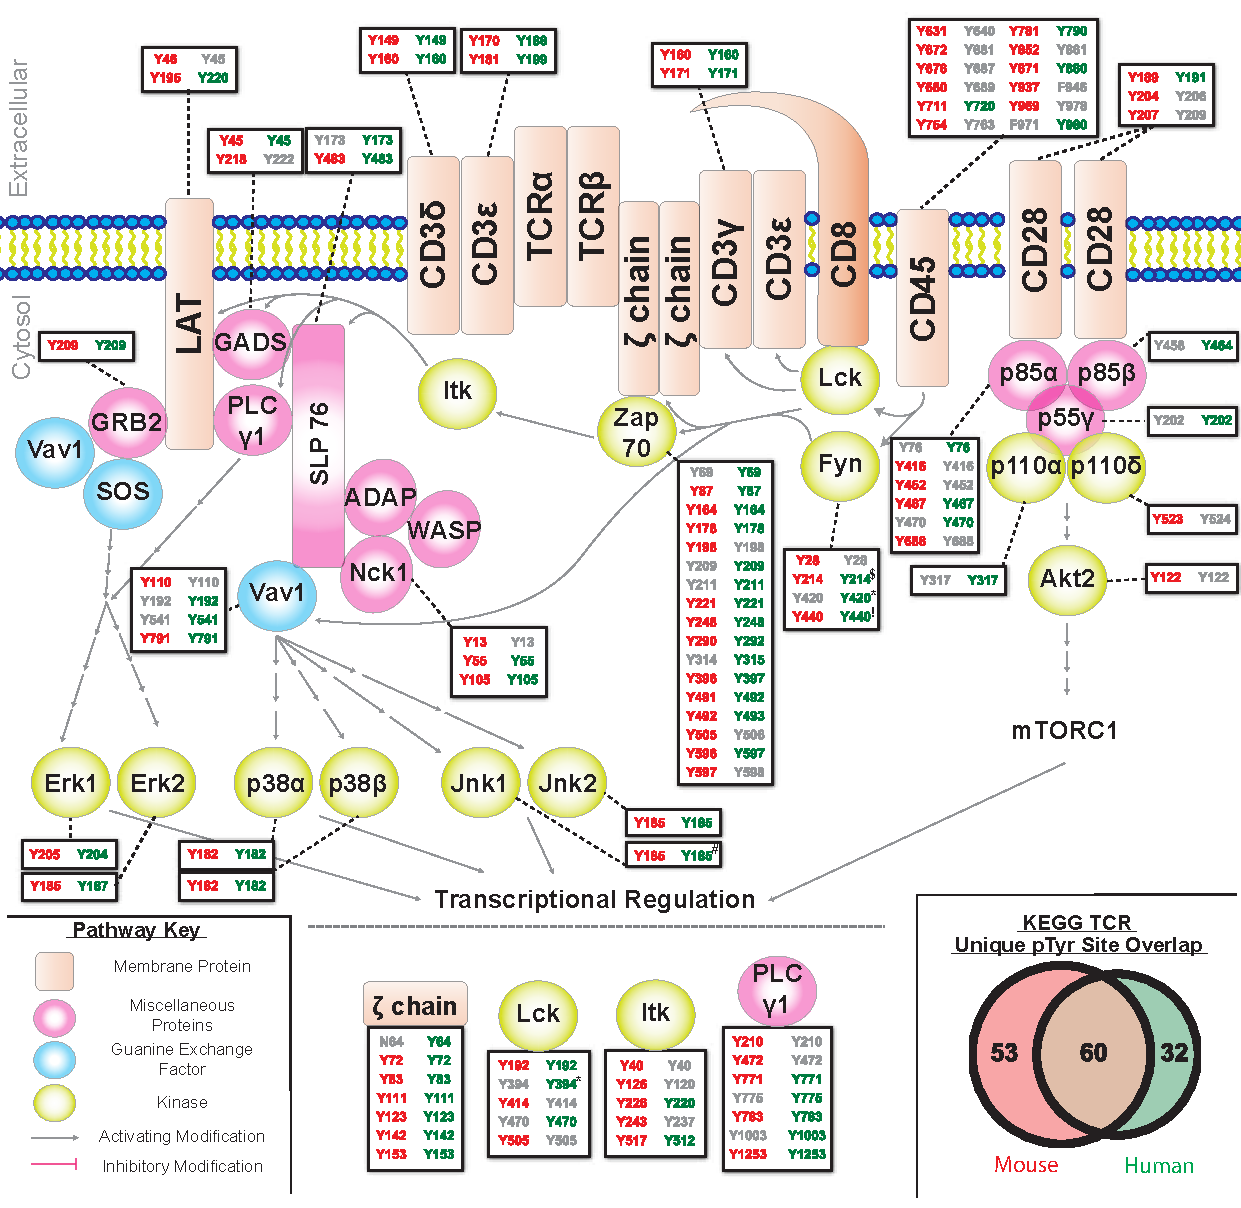
\includegraphics[width=170mm]{figures/main_figs/biologically_interesting.pdf}
\caption{BOOST pTyr proteomics reveals a comparable number of unique TCR-related pTyr sites in primary T cells from mice and Jurkat T cells. Unique pTyr sites identified in our BOOST experiment with the $\Phi$SDM disabled are colored in red. Unique pTyr sites identified by \citeauthor{chua2020tandem} \citeyear{chua2020tandem} in the Jurkat T cell model system for studying TCR signaling are colored in green. Inset shows the overlap between unique pTyr sites in the Kyoto Encyclopedia of Genes and Genomes T cell receptor signaling pathway between our BOOST experiment and the BOOST experiment performed by \citeauthor{chua2020tandem} \citeyear{chua2020tandem}. Special characters next to site numbers indicate the presence of PSMs that arise from multiple proteins:  $^{\textbf{\$}}$Fyn/Yes1 $|$ $^{\textbf{*}}$Fyn/Yes1/Src/Lck $|$ $^{\textbf{!}}$Fyn/Yes1/Src $|$ $^{\textbf{\#}}$Jnk1/Jnk3.  }\label{biologically_interesting}
\end{figure}

To show the efficacy of BOOST pTyr proteomics in primary T cells we used $\alpha$-CD3 antibodies to stimulate TCR signaling (Figure \ref{experimental_design}). Therefore, we expected to observe many unique pTyr sites on TCR signaling proteins. In accordance with our expectations, we observed a total of $113$ unique pTyr sites on proteins in the Kyoto Encyclopedia of Genes and Genomes (KEGG) T cell receptor signaling pathway (Figure \ref{biologically_interesting}, Supporting Figure $15$). To determine the profiling range of unique pTyr site sequencing in primary T cells using BOOST, we compared our BOOST experiment with the $\Phi$SDM disabled to our previously published BOOST experiment in Jurkat T cells which used an equivalent amount of cellular protein and set of contrived ratios ($1.0$:$0.3$:$0.1$ mg total protein)\cite{chua2020tandem}. Our Jurkat BOOST experiment was acquired using an Orbitrap Fusion Lumos Tribrid mass spectrometer without the $\Phi$SDM and had a similar BOOST-gained yield to the present primary T cell BOOST data\cite{yu2020benchmarking,chua2020tandem}, and is therefore suitable for comparison. Within the KEGG TCR annotated proteins, we observed $60$ pTyr sites in both mouse and Jurkat BOOST experiments (Figure \ref{biologically_interesting} inset, Supporting Figure $15$), with the majority of these sites on ITAMs (TCR$\zeta$, CD3$\delta$/$\epsilon$/$\gamma$; $12$), the tyrosine kinase Zap70 ($10$), and the canonical activation sites on mitogen activated protein kinases (Erk1/2, p38$\alpha$/$\beta$, Jnk$1/2/3$; $7$). We found $53$ unique pTyr sites exclusive to BOOST in primary T cells from mice, compared to $32$ unique pTyr sites exclusive to BOOST in Jurkat T cells (Figure \ref{biologically_interesting} inset, Supporting Figure $15$). Notably, using the BOOST method in primary T cells from mice uncovered $8$ pTyr sites on CD45, a phosphatase critical for the activation of Lck\cite{sieh1993cd45}, and $4$ pTyr sites on Tec, a non receptor tyrosine kinase with overlapping function with Itk in TCR signaling\cite{yang1999role,aoki2004mutual}. Of the $4$ unique pTyr sites observed on Tec, the activation site (Y519) was quantified in all three replicates in the $1.0$, $0.3$, and $0.1$ mg samples of the BOOST experiment, whereas it was quantified in some but not all replicates of all conditions of the $1.0$ mg Control experiment. Similar results were found for SHP-1$^{\text{Y536}}$, Itk$^{\text{Y512}}$, Zap70$^{\text{Y290}}$, and Zap70$^{\text{Y492}}$ from our BOOST experiment in primary T cells from mice (Supporting Table $2$). These results suggest that using BOOST in primary T cells from mice increases pTyr profiling depth similarly to what we observed previously using Jurkat T cells\cite{chua2020tandem,chua2021ovalbumin}.

\section{Discussion}

To improve our understanding of the critical tyrosine phosphorylation events involved in TCR signaling and other cellular processes, accurate methods to perform deep profiling of the pTyr proteome are required. Although the accuracy of LC-MS/MS techniques are desirable for pTyr proteomics, the low abundance of tyrosine phosphorylation events in the proteome hinder the frequently used global phosphoenrichment methods like TiO$_{2}$ or IMAC\cite{navarro2011phosphoproteomic,prado2021synergistic,thingholm2006highly,thingholm2016use,thingholm2016phosphopeptide}. Although recent developments in pTyr-specific enrichment techniques like p-Tyr-1000 and the superbinder SH2 method have improved pTyr proteomics\cite{kaneko2012superbinder,bian2016ultra,dong2017sensitive,tong2017protein,yao2018sh2,yao2019one,chua2020tandem}, the issue of low pTyr abundance is apparent when using samples that are difficult or expensive to collect, such as primary cells from humans or mice\cite{salter2021comparative,ramello2019immunoproteomic,locard2020lymphoatlas}. Increasing quantitative yield in low abundance samples has been acheived in multiplexed TMT experiments using a carrier proteome sample\cite{petelski2021multiplexed,stopfer2021quantitative,cheung2021defining}, and we developed the BOOST method using a pervanadate treated sample to increase quantitative yield of pTyr peptides\cite{chua2020tandem,chua2021ovalbumin}.

 Here, we demonstrate the first use of the BOOST method in primary T cells from mice, defining the accuracy, precision, and profiling depth of the mouse T cell pTyr proteome in low abundance samples. Our multiplexed TMT experiments were designed to minimize reporter ion interference from the pervanadate channel by including a ``Blank" (127C) channel where maximal reporter ion interference has been observed previously (Supporting Figures $3$-$6$, Figure \ref{depth_nans})\cite{chua2021ovalbumin,stopfer2021quantitative}. Using BOOST, we were able to quantify more than $2{,}000$, $900$, and $300$ unqiue pTyr peptides in $1.0$ mg, $0.3$ mg, and $0.1$ mg protein samples, respectively (Figure \ref{depth_nans}D), while maintaining accuracy and precision (Figure \ref{accuracy_and_precision}, Supporting Figure $4$). Using BOOST allowed for $3{,}006$ BOOST-gained pTyr peptides to be quantified with $2{,}939$ pTyr peptides that were low abundance in the samples (Figure \ref{boost_factor}C). This included $113$ unique pTyr sites on proteins involved in the T cell receptor signaling pathway, with $53$ of these sites being uniquely identified in mice when compared to our the pTyr sites we originally identified in Jurkat T cells (Figure \ref{biologically_interesting}, Supporting Figure $12$)\cite{chua2020tandem}. Of the TCR signaling proteins indentified using BOOST, many of the unique pTyr sites were found in all replicates of the $0.3$ and/or $0.1$ mg samples in the BOOST experiment and not in the $1.0$ mg Control experiment. Together, our data suggest that including a pervanadate BOOST channel increases quantitative depth of low abundance peptides in higher abundance samples and overall quantitation in low abundance samples without large comprimises to accuracy or precision while increasing the number of significant changes observed in the tyrosine phosphoproteome.

We also examined the influence of the acquisition parameter $\Phi$SDM, a computational method that increases acquisition rate of FT-MS by efficient and noise tolerant deconvolution of FT spectra\cite{grinfeld2017phase}, on our BOOST and $1.0$ mg Control samples. Although previous research has shown that using the $\Phi$SDM on long gradients or scarce samples may reduce the efficiency of the algorithm due to low ion currents\cite{grinfeld2017phase,yu2020benchmarking,kelstrup2018limits}, the influence of the $\Phi$SDM on TMT mixes with carrier proteome channels has yet to be evaluated. Our data are in agreement with previous literature suggesting that enabling the $\Phi$SDM degrades low abundance samples. We observed a decrease of about $75$ to $100$ unique pTyr peptides across our $1.0$ mg Control samples with the $\Phi$SDM enabled, with the largest loss in the $0.1$ mg R1 sample ($221$ to $104$ unique pTyr peptides; Figure \ref{depth_nans}A,B). Surprisingly, enabling the $\Phi$SDM degraded the quality of data from BOOST experiments. We observed a large reduction of unique pTyr peptide yield in experimental channels, with the largest difference being $1.0$ mg R1 dropping from $2{,}931$ unique pTyr peptides to $784$ unique pTyr peptides with the $\Phi$SDM enabled (Figure \ref{depth_nans}C,D). We also observed a reduction in accuracy (Figure \ref{accuracy_and_precision}B), precision (Figure \ref{accuracy_and_precision}C), and replicate reproducibility (Supporting Figures $4$, $5$) with the $\Phi$SDM enabled. Our study indicates that disabling the $\Phi$SDM, or ``Turbo-TMT" on the method editor on Orbitrap instruments, subtstantially improves the quantitation depth of low abundance posttranslational modification samples, especially when a BOOST channel is present.

With increased interest in using proteomics to study rare or specific posttranslational modifications\cite{millan2020histone,yao2019one,fulzele2018ubiquitin} and the proteomes of single-cells\cite{petelski2021multiplexed,cheung2021defining,vistain2021single}, reliable methods to increase multiplexing capabilities\cite{arul2018sample}, posttranslational modification selection\cite{pieroni2020enrichments}, and quantitation\cite{chua2020tandem,chua2021ovalbumin,pino2020acquiring} are desired. These experimental techniques will come with a wave of computational methods to further improve quantitation\cite{grinfeld2017phase,sinitcyn2021maxdia,bilbao2018algorithm}, which will require stringent testing for both experimental-computational method compatibility and to understand the range of biological processes that these methods can work with. In this study, we displayed both of these features for the BOOST method by showing that BOOST and the $\Phi$SDM were incompatible and that BOOST can increase the yield of pTyr peptides in primary T cells from mice, which are notoriously refractory for wide scale analysis\cite{locard2020lymphoatlas}. By using this study as a benchmark for the BOOST method in primary T cells from mice, future research into the pTyr proteome of primary T cells from mice is possible using far less sample than is conventionally used.


\section{Conclusion}

Our study defines the accuracy, precision, and profiling depth of multiplexed TMT experiments using a pervandate BOOST channel to increase quantitative yield of pTyr peptides in stimulated primary T cells from mice. We found that including the BOOST channel increases the quantitative yield of unique pTyr peptide PSMs without jeoprodizing accuracy, precision, or replicate reproducibility in low abundance samples. Importantly, we found no evidence of reporter ion interference in experimental channels or ratio compression when using BOOST and SPS-MS3 quantitation. The majority of the unique pTyr peptide PSMs observed in the BOOST channel and at least one experimental channel were scarce in the samples, suggesting that BOOST increases identification of rare pTyr peptides. Interestingly, we found that enabling the $\Phi$SDM degrades the quality of data in BOOST experiments, almost halving the unique pTyr peptide PSM yield and reducing accuracy, precision, and replicate reproducibility in low abundance samples. Using BOOST, we were able to quantify many unique pTyr sites on proteins involved in TCR signaling in experimental channels. Together, our study shows that multiplexed TMT experiments using a pervanadate BOOST channel increase quatitative yield of meaningful unique pTyr peptide PSMs in primary T cells from mice and that the $\Phi$SDM should be avoided for BOOST experiments.

\section{Supporting Information}

The Supporting Information is available free of charge at \href{https://pubs.acs.org/}{https://pubs.acs.org/}. Supporting Information includes:

\begin{itemize}
    \item {All tables generated after MaxQuant analysis of .raw files (``summary.txt", ``evidence.txt", ``peptides.txt", ``modificationSpecificPeptides.txt", ``Oxidation (M)Sites.txt", ``Phospho (STY)Sites.txt", ``proteinGroups.txt", ``allPeptides.txt", ``msScans.txt", ``mzRange.txt", ``msmsScans.txt",  and ``msms.txt") (.ZIP)}
    \item {All Python3 code used to perform data analysis and representation, including statistical analyses, replicate reproducibility assessments, BOOST factor analysis, and comparisons between TMT experiments (.ZIP)}
    \item {All output from statistical analyses performed and selected MaxQuant output required for statistical analysis (.XLSX)}
\end{itemize}

\section{Acknowledgements}

The authors wish to thank Dr. Ricky Edmondson and Dr. Samuel G. Mackintosh from University of Arkansas for Medical Sciences (UAMS) for collecting the proteomic data. We acknowledge financial support from NIH grants R01AI083636, P20GM121293, and R24GM137786. Kenneth P. Callahan was supported by T32GM136566 and the Sidney E. Frank Fellowship.

\section{Data Availability}

The mass spectrometry proteomic data have been deposited to the ProteomeXchange Consortium (\href{http://proteomecentral.proteomexchange.org}{http://proteomecentral.proteomexchange.org}) via the PRIDE partner repository\cite{vizcaino2012proteomics} with the dataset identifier PXD025853 (Username: reviewer\_pxd025853\@ebi.ac.uk , Password: RDtiS7iG).  


\bibliography{citations.bib}

\end{document}